 
\section{Our focus and plan}

% % % TODO % % % %
%from rules: Innovative technology (if any) TODO describe usage of STRANDS
%from rules: Reusability of the system or parts thereof - see STRANDS
This section summarises our intentions for our system this year. We would like to aim for high re-usability of code in our robotic system and to demonstrate that the current state of the art in AI algorithms mixed with our extensions can be successfully used to produce a robust, effective and complete robotic system with domestic applications.  

\subsection{Catering for Granny Annie’s Comfort}

A robot will receive commands from Granny Annie by natural speech. These commands may contain interaction with an intelligent flat or bringing to her a specific object. 
We have not participated in this task last year because we had not a robust speech recognition as neither of us is an expert in the field. 
However, we have started a cooperation with research group in this field and we hope to be able to recognise speech more robustly than using CMU Sphinx last year, see Sec.~\ref{sec:speechrec}.

We would like to prepare our robot so that it can perform the first part - cooperation/interaction with an intelligent flat. This subtask still contains interesting challenges, such as robust speech recognition and robot navigation in a way, which is comfortable and natural for a human.  

%The problem of speech recognition is often discussed within the robotic community. It is something, which is necessary for future robots to cooperate with humans. Assuming a robot is working at Granny's flat, the robot can learn and adapt to her voice, which will increases its performance over time. Moreover, Granny is living alone, thus, it can be assumed that the level of background noise is minimal. In contrast, during the competition, speech recognition provides a lot of challenges. The background noise is really high during competition because of the spectators. Furthermore, the person playing Granny Annie changes, hence a robot cannot improve its behaviour. 



%The second part of this task - bringing someone a specific object - is even more challenging as it includes two large robotics domains, computer vision and manipulation. As our robot has no manipulator this year (see Section \ref{sec:hardware}), we might be able to perform only object search. We might benefit from experiences from a previous project in our robotic group - CogX \cite{cogx}. In this project, one of the robot's abilities was to search for known objects by taking into account common sense knowledge (i.e. prior knowledge) in the form of probabilities of objects' presence in different rooms. However, this will still require a lot of effort from us, as the robot was not using ROS before and we will need to understand and integrate bits into our system. We assume to work on this part next year.

\subsection{Welcoming visitors}

In this task, a robot should welcome visitors, recognise them and accompany them to a specific location in Granny's flat. Several components are needed in this task: computer vision for face recognition and for uniform detection. Moreover, machine learning techniques are needed to be able to learn these two patterns in order to recognise them. A robot can also benefit from speech recognition if face/uniform recognition does not provide a certain decision. Additionally, a robot must have robust navigation in an environment in order to accompany a person to a specific place. 
Finally, human-robot interaction is needed while accompanying a person.

Last year, we successfully completed this task. Our system was built on several components which are mentioned in Sec.~\ref{sec:software}. 
Here, we would like to discuss their properties, advantages and disadvantages and their future extensions. 
Our core state machine is built for this task calling several components. 
We do not plan changes in our face recognition system as neither of us is an expert in this field. 
However, we will create bigger database of faces in order to support machine learning algorithm.

Uniform recognition needs to be improved due to following reasons.
First, recognition was based on manual sensitive calibration of colours last year, which slowed down preparation and the calibration was sometimes impossible. 
Second, uniform detection was based only on segmentation of all the picture. This means, if there is significantly big object of certain colour belonging to an uniform (white/yellow) in the background, this object will be classified as the person. 
Both issue were limitations last year and we are improving them.  

The last issue of our system last year was not sufficient detection of a human. Thus, our human-robot interaction was strongly limited. 
We were using only a leg detector based on the readings from the laser scanner. 
This system was not robust enough. 
Hence we are testing how to combine this system with an upper-body detector based on a depth camera or an IR camera.

\subsection{Getting to know my home}

In this task, a robot should recognise changes in a flat, such as open/closed doors, furniture has been moved to another room or everyday objects were moved. 
The robot can detect these changes autonomously or by cooperation with a human who used speech or gestures.
After detection, the robot is asked to use this new knowledge to execute some commands, such as to bring a mug on the dining table which is now in living room.

The state machine for this task from last year is in Fig.~\ref{fig:st1}.
Our system was built on two parts - autonomous detection of doors using the laser rangefinder and cooperation with human in order to detect where is furniture. 
 However, the robot was unable to detect exact position of the furniture which is important to be able to use the knowledge later. 
Therefore, we would like to integrate one of the STRANDS packages this year, which is able to detect dynamic clusters from 3D point clouds and recognise to which object they belong. 
Additionally, we would like to detect objects as well.

Finally, we used CMU Sphinx last year for speech recognition. 
However, this system is not proper for this usage due to limited dictionary and usage. 
Therefore, we are going to change our speech recognition system, see Sec.~\ref{sec:speechrec}.

\begin{figure}[!htb]
\centering
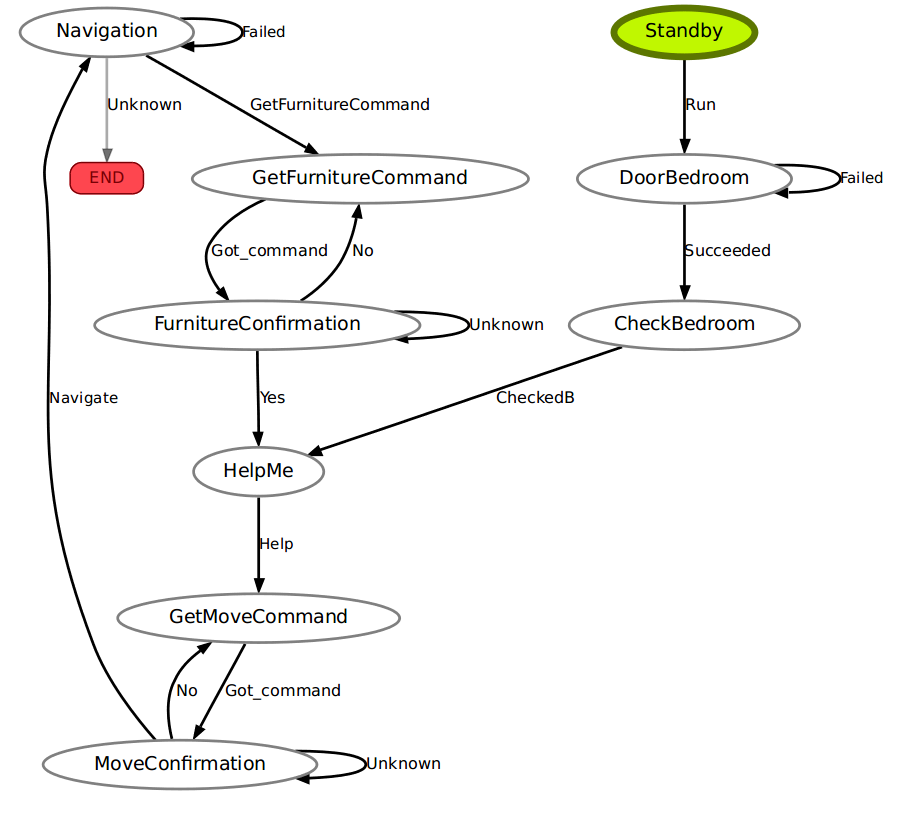
\includegraphics[width=3.in]{statemachine_t1.png}
\caption{The state machine for task Getting to know my home}
\label{fig:st1}
\end{figure}

\subsection{Object perception} 

We are currently comparing two different approaches for object detection and recognition. The first approach uses manually created point-cloud models with rgb information. 
The advantage is that this algorithm detects the exact objects which were used for training. 
%TODO slovicko occluded ???
However, if the object is occluded then the detection is significantly worse.
Additionally, this approach is possible for a small set of object because each object needs manually created model. 

In contrast, the second approach uses a database of 3D models of objects. These object do not represent any specific object, they rare created in software for 3D visualisation to represent a general object. 
Hence, the second approach uses such database to train knowledge how general chair, mug, banana, etc. looks like. 

We are additionally evaluating an approach which uses transfer learning to recognise objects using a convolutional neural network (CNN) which has been pre-trained for another task, in our case, image classification \cite{schwarz}. An RGB-D pair of images is first pre-processed as shown in Fig.~\ref{fig:object_perception}. Next, the images are processed by the CNN in order to extract a vector of image features for each RGB-D frame. This feature vector is used with a tree of classifiers and regressors to determine first the category of the object, then the object instance, and finally the pose of the object.

\begin{figure}[!htb]
\centering
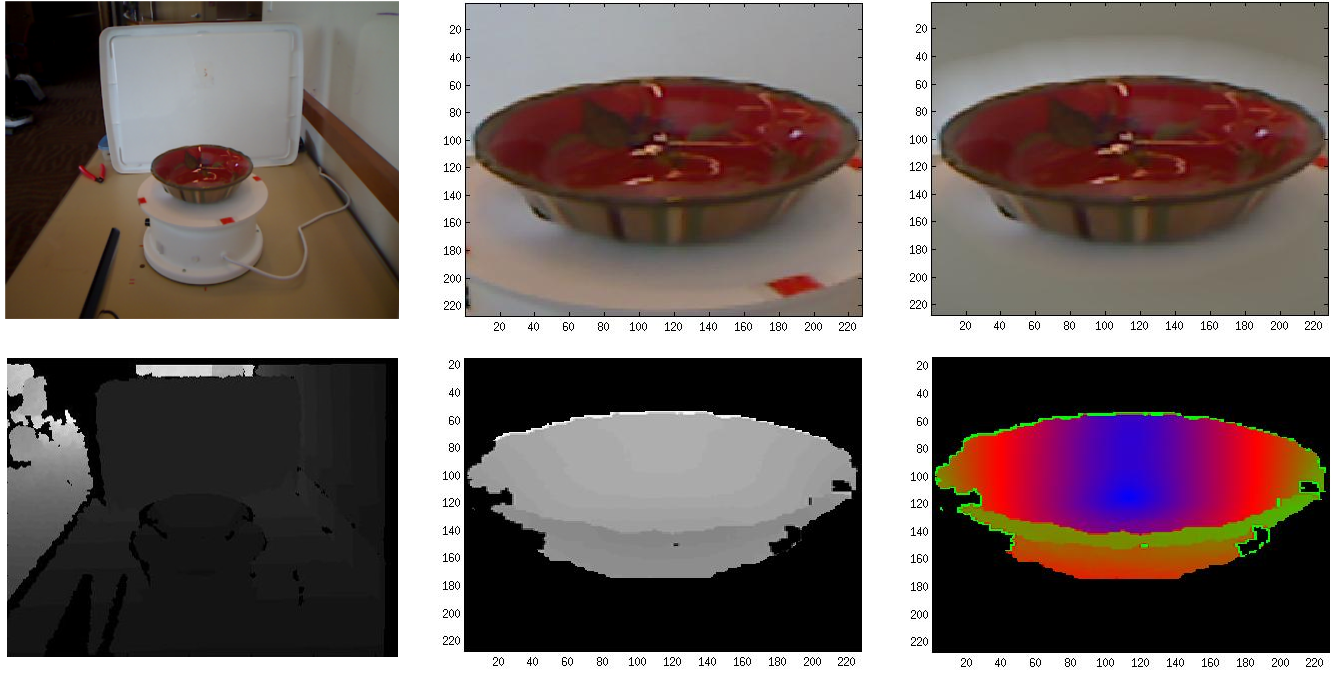
\includegraphics[width=3.in]{object_perception.png}
\caption{The image pre-processing pipeline for the described algorithm. Top: The RGB image is first cropped down to size and then a fading algorithm is used to reduce the chance of unwanted features being detected in the background of the image. Bottom: The depth image is cropped in the same way and then coloured based on the depth data. This is required because the CNN is trained to detect features in RGB images and so we want the new image to describe the depth information in RGB.}
\label{fig:object_perception}
\end{figure}

\subsection{Navigation}

We had robust configuration of navigation stack from ROS last year, which combined benefits from laser rangefinder and a depth camera. 
Additionally, we have added monitored navigation to recover from failure and topological navigation in order to control behaviour of the robot in different rooms. Details are explained in Sec.~\ref{sec:software}.

\subsection{\label{sec:speechrec}Speech understanding}

Last year, we used CMU Sphinx for speech recognition with no added microphone. CMU Sphinx is not good enough for this benchmark. 
Therefore, we have started to cooperate with research group of speech recognition in our faculty in order to deploy more sophisticated algorithm on our robot. 
Unfortunately, no details are known yet, as the work on this benchmark will start in September.

\subsection{Timetable}

We are doing our best in order to participate in all tests. However, our priorities are following.
First, we will perform complete \textit{Welcoming visitor} task. 
Moreover, we will detect not only doors changes, but also precise locations of furniture in \textit{Getting to know my home} task. 
We will participate in \textit{Navigation} benchmark. We hope to participate in the rest of tasks, but it is depend if we will be able to recruit new team members.


%\begin{figure}[!htb]
%\centering
%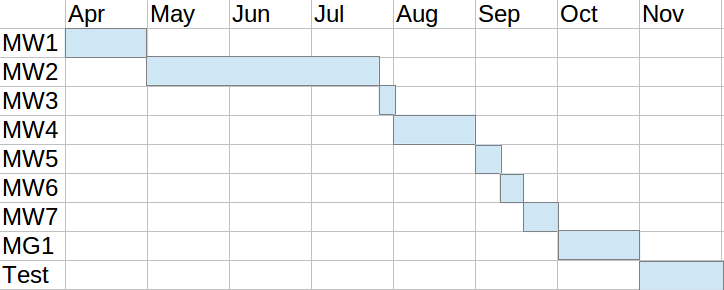
\includegraphics[width=3.in]{timetable.png}
%\caption{Timetable}
%\label{fig:plan}
%\end{figure}
